\documentclass[
      english,
			conference,
      ]{IEEEtran}

\usepackage{flushend}
%% ======================== SETUP =========================
%% Full documentation on all packages can be found at http://google.com or with `texdoc <packagename>`


%% === Tools ==============================================
\usepackage{iftex}
\usepackage{savesym}
%%   - Silence -
%% Disable warnings that don't cause problems
\usepackage{silence}
\WarningFilter{balance}{You have called \balance in second column}
\WarningFilter{caption}{Unsupported document class}
\WarningFilter{caption}{Unused \captionsetup}
\WarningFilter{relsize}{Failed to get list}


%% === Encoding ===========================================
\ifXeTeX
  \usepackage{fontspec}
\else
  \usepackage[utf8]{inputenc}
  \usepackage[T1]{fontenc}
  \input glyphtounicode			%% Copyable unicode in pdf
  \pdfgentounicode=1
\fi


%%% === ACM Template =======================================
%%% Depending on font, may look better with `relayout`
%\usepackage[relayout]{myacm}
%\usepackage{balance}
%%%   - Default font, choose one -
%\usepackage{txfonts}			%% Times Roman, as requested by style guide, creates smaller documents
%%\usepackage[lighttt]{lmodern}	%% Latin Modern, with light typewriter, looks almost like default setting


%% === article Template ===================================
%%   - Font -
\usepackage[lighttt]{lmodern}	%% Latin Modern with light typewriter


%% === Fonts ==============================================
%%   - Other -
%\savesymbol{iint}					%% Better math font
%\savesymbol{iiint}				%
%\savesymbol{iiiint}				%
%\savesymbol{idotsint}			%
\usepackage{MnSymbol}			%% /Better math font
\usepackage[babel=true]{microtype} %% Better kerning


%% === Language ===========================================
\usepackage{babel} 							%% Select language in \documentclass
\usepackage[babel]{csquotes}		%% \enquote, \blockquote
%%   - Quotes -
%% Options for english: british -> '', american -> ""
\ExecuteQuoteOptions{french=guillemets,german=quotes,english=american}
\newcommand\q[1]{\enquote{#1}}	%% Quote with \q{}
\MakeAutoQuote{>}{<} %% {«}{»}
\MakeOuterQuote{"}


%% === Page Format ========================================
%\usepackage{fancyhdr}			%% more header and footer configuration
%\usepackage{pdflscape}			%% \begin{landscape} ... \end{landscape}


%% === Bibliography =======================================
%% use biblatex if you know what you're doing
%\usepackage[
		%%backend=bibtex, 			%% bibtex, no utf-8 support
		%backend=biber,				%% biber backend
		%style=numeric-comp,		%% [1]
		%%style=alphabetic, 		%% [Auth99]
		%%citestyle=authortitle-tcomp,
		%%bibstyle=verbose,
		%%backref=true,
		%defernumbers=true,
		%doi=false,isbn=false,url=false,
		%]{biblatex}
		
		
%% === Images =============================================
\usepackage{graphicx}			%% \includegraphics
\usepackage{subfig}				%% Sub-figures
\DeclareGraphicsExtensions{.pdf,.png,.jpg,.ai}
\DeclareGraphicsRule{.ai}{pdf}{*}{}


%% === Colors =============================================
\usepackage{color}
%\usepackage{colortbl}					%% Colors for tables
\usepackage[svgnames,table]{xcolor}		%% more colors and \rowcolors


%% === Tables =============================================
%\usepackage{ctable}				%% \ctable command
%%  - Table Style -
%% colored rows, requires xcolor
%\newcommand{\insidetable}{\rowcolors*{2}{WhiteSmoke}{white}}
%\setupctable{doinside=\insidetable}


%% === Code Listings ======================================
\usepackage{listings}
%%   - Basic Looks -
\lstset{
	captionpos=b, 
	xleftmargin=0.35cm,
	basicstyle=\smaller\ttfamily, 
	showstringspaces=false, 
	columns=fixed, 
	basewidth={0.5em,0.45em}, 
	upquote=true,
	tabsize=2, 
	gobble=2,
	escapeinside={/*@}{@*/},
	numberbychapter=false,
}
%%   - Linebreaks -
\lstset{
	breaklines=true, 
	breakatwhitespace=true,
	%prebreak=\raisebox{0ex}[0ex][0ex]{\emptyaccsupp{\small\ensuremath{\rhookswarrow}}},
	postbreak=\raisebox{0ex}[0ex][0ex]{\emptyaccsupp{\small\ensuremath{\rcurvearrowse\space}}},
}
%%   - Line Numbers -
\lstset{
	numbers=left, 
	numberstyle=\tiny\emptyaccsupp, 
	numbersep=5pt,
	numberfirstline=true, 
	firstnumber=auto, 
	stepnumber=5,
}
%%   - Copy&Paste -
\lstset{keepspaces=true}
\ifXeTeX
\else
  \makeatletter
  \def\lst@outputspace{{\ifx\lst@bkgcolor\empty\color{white}\else\lst@bkgcolor\fi\lst@visiblespace}}
  \makeatother
	\pdfglyphtounicode{visiblespace}{A0}
	\pdfglyphtounicode{blank}{A0}
	\pdfglyphtounicode{visualspace}{A0}
	\pdfglyphtounicode{uni2423}{A0}
\fi
%%   - Languages -
\lstdefinelanguage{JavaScript}{
	keywords={break, case, catch, continue, debugger, default, delete, do, else, finally, for, function, if, in, instanceof, new, return, switch, this, throw, try, typeof, var, void, while, with},
	morecomment=[l]{//},
	morecomment=[s]{/*}{*/},
	morestring=[b]',
	morestring=[b]",
	sensitive=true,
}
\lstdefinelanguage{HanaSQL}[]{SQL}{
	morekeywords={replace,string,if,daysbetween,secondsbetween,weekday,adddays,addseconds,double},
}
\lstdefinelanguage{algorithm}{
	keywords={break, case, catch, continue, dec, default, delete, do, each, else, end, error, exists, finally, for, function, if, inc, is, new, return, switch, then, this, throw, try, typeof, until, var, void, while, with},
	morestring=[b]",
	morecomment=[l]{//},
	morecomment=[s]{/*}{*/},
	moredelim=[is][\slshape]{'}{'},
	moredelim=[is][\bfseries]{''}{''},
	style=algorithmStyle,
}
\lstdefinestyle{algorithmStyle}{
  literate= % replace with math symbols
			{:=}{{\(\gets\)}}2 {~}{{\(\:\!\!\neg\)}}1
			{<=}{{\(\leq\)}}1 {>=}{{\(\geq\)}}1 
			{!=}{{\(\neq\)}}1 {=}{{\(=\)}}1
			{&&}{{\(\wedge\)}}1 {||}{{\(\vee\)}}1 
			{\{\}}{{\(\emptyset\)}}1
			{\\in}{{\(\in\)}}1
			{\\notin}{{\(\notin\)}}1
			{\\exists}{{\(\exists\)}}1
			{\\nsubseteq}{{\(\subseteq\)}}1
			{<<}{{\(\ll\)}}2
			% escape with \
			{\\:=}{{:=}}2 {\\~}{{\textasciitilde}}1
			{\\<=}{{<=}}2 {\\>=}{{>=}}2 
			{\\!=}{{!=}}2  {\\=}{{=}}1
			{\\&&}{{\&\&}}2 {\\||}{{||}}2 
			{\\\{\}}{{\{\}}}2
			{\\bs}{{\textbackslash}}1 
			{\\'}{{'}}1 
}
%%   - Styles -
\lstdefinestyle{EclipseStyle}{
	keywordstyle=\bfseries\color{Purple},
	stringstyle=\color{Blue},
	commentstyle=\color{Grey},
}
\lstdefinestyle{BWStyle}{
	keywordstyle=\bfseries,
	stringstyle=\color{DimGray},
	commentstyle=\slshape,
}
\lstset{style=BWStyle,language=Java}
\lstMakeShortInline[basicstyle=\ttfamily,language={}]´


%% === More Tools =========================================
%% no changes here
\usepackage{xspace} 			%% \xspace, automatic spaces for custom macros
\usepackage{float}				%% custom floats
\usepackage{mparhack}			%% marginpar hack
% \usepackage{fixltx2e}			%% latex bugs
\usepackage{relsize}			%% \smaller
\usepackage[space=true]{accsupp}
\newcommand\emptyaccsupp[1]{\BeginAccSupp{ActualText={}}#1\EndAccSupp{}}


%% === Misc ===============================================
\usepackage[printonlyused]{acronym}	%% Acronyms
\renewcommand*{\acsfont}[1]{\textsc{#1}}
%% pdfcomments, load before hyperref
\usepackage{pdfcomment}
%% Exclude footnote links from copy&paste
\renewcommand{\thefootnote}{\protect\BeginAccSupp{ActualText={}}\arabic{footnote}\protect\EndAccSupp{}}


%% === Links and Captions =================================
%\usepackage{hyperref}
%\hypersetup{
%%	draft,						%% disable all
	%%% better set this as document option
	%%colorlinks, 				%% color links, instead of bordered
	%hidelinks,					%% for print version
%%% - link colors -
	%linkcolor=Navy,				%% internal, default red
	%citecolor=Navy,				%% citations, default green
	%urlcolor=Purple,			%% URLs, default cyan
	%filecolor=Purple,			%% files, default magenta
%%
	%plainpages=false,
%}

\usepackage[nameinlink, noabbrev]{cleveref}	%% \cref commands
\newcommand{\lineref}[2]{\hyperref[#1]{line~\ref*{#1:#2}}}
\newcommand{\linerefn}[2]{\hyperref[#1]{line~#2}}
\newcommand{\Lineref}[2]{\hyperref[#1]{Line~\ref*{#1:#2}}}
\newcommand{\Linerefn}[2]{\hyperref[#1]{Line~#2}}

%\usepackage[all]{hypcap}
%\usepackage{caption}
%\captionsetup[table]{position=t}
%\captionsetup[subtable]{position=t}


%% === Misc 2 ============================================
\usepackage[xspace]{ellipsis}	%% \dots, load after hyperref


%% === Pdf Options =======================================
\hypersetup{
	draft
	%bookmarksopen,
	%bookmarksnumbered,
%%	pdfstartview={Fit},					%% Fit page
%%	pdfstartview={FitH},				%% Fit width
	%pdfstartview={XYZ null null 1.0},	%% 100% zoom
}

%\bibliography{references}

\title{Back-in-Time Debugging in \\Heterogeneous Software Stacks}

\author{\IEEEauthorblockN{Arian Treffer}
\IEEEauthorblockA{Hasso-Plattner-Institut\\
Potsdam, Germany\\
Email: arian.treffer@hpi.de}
\and
\IEEEauthorblockN{Matthias Uflacker}
\IEEEauthorblockA{Hasso-Plattner-Institut\\
Potsdam, Germany\\
Email: matthias.uflacker@hpi.de}
}



\hypersetup{
	pdftitle={},
	pdfauthor={Arian Treffer, Matthias Uflacker},
	pdfsubject={},
}

% remove in final version
%\usepackage[colorinlistoftodos]{todonotes}
%\renewcommand{\todo}[2][\empty]{\pdfmargincomment[color=orange,icon=Note,subject=TODO,#1]{#2}}
%\usepackage{pdfcomment}
%\newcommand{\todo}[2][]{\pdfmargincomment[color=orange,icon=Note,subject={TODO},author={#1}]{#2}}

\begin{document}

\maketitle

\begin{abstract}
Back-in-time, or omniscient debuggers can help developers to debug software more efficiently. However, complex business applications often consist of multiple components that run in distinct systems or environments, were developed in different programming languages, and require separate debugging tools.
We interviewed five developers of business applications to understand how such software is developed and debugged. Based on these insights we developed a prototype back-in-time debugger that allows developers the seamless debugging of the entire stack of a 3-tier application, from the front-end running in the browser down to stored procedures in the database.
High-level visualizations guide the developer in understanding the relations between sub-systems and help to sequentially debug concurrent requests. We evaluated our approach with a real-world project. Encouraged by promising developer feedback, we discuss steps to generalize our work into a debugger for arbitrary heterogeneous software systems.
\end{abstract}

\section{Introduction}
\label{sec:introduction}

% Context: architectures
Complex applications are rarely single programs running on a single machine but often consist of multiple components implemented in different programming languages and running in different environments.
A notable example is the multi-tier architecture, a successful and established pattern for client-server applications since over two decades.

% Problem
Breaking down applications into layers and sub-systems allows for better scalability and easier life-cycle management, but makes debugging such applications much harder.
Software failures are typically observed in the front-end first.
Then, developers have to guess which layer contains the fault. 
Otherwise, they have to switch debugging tools frequently while they track the infection chain across the entire software stack.

% Signifiance
In the past, this problem was mitigated because most application code resided in the business tier, while the presentation and data tiers only served to display back-end provided views and to persist application state, respectively.
However, changes in technologies and requirements caused more code to move up or down the stack, thereby increasing the need to debug the application as a whole.
Service-oriented architecture and micro-services are more recent patterns that exacerbate the problem by dividing applications into even more independent components.

% Solution
We interviewed software developers on the difficulties when developing modern enterprise applications.
Based on these insights, we developed a prototype for a back-in-time debugger allowing developers to debug the full stack of a 3-tier application in one session.

Assuming back-in-time debugging capabilities for each application tier, we introduce hierarchical step numbering based on synchronization points between components to create a partial ordering of instructions in all concurrent executions.
A visualization shows which UI element is affected by which back-end operation, providing developers with a top-down summary of the execution.
A second visualization is shown in the debugger and helps developers to navigate the application flow.

We then collected developer feedback for our prototype.
Based on this feedback, we identified suggestions how existing debugging tools can be improved even without the need for resource-intensive back-in-time debugging.

The remainder of this paper is structured as follows:
The next section summarizes related work.
\Cref{sec:interviews} discusses the results of our interviews. 
We describe in more detail how 3-tier applications have changed in the last decade and which information developers need when debugging such applications.
\Cref{sec:debugger} presents our prototype implementation of a full-stack back-in-time debugger.
\Cref{sec:conclusion} concludes.

\section{Related Work}

%The concept of slicing was introduced by Weiser and initially only built on static analysis \cite{weiser_programmers_1982, weiser_program_1981}.
%Later, Korel and Laski \cite{korel_dynamic_1990} and Agrawal and Horgan \cite{agrawal_dynamic_1990} introduced dynamic slicing by proposing different ways of extending the concept to the run-time.

The idea of being able to debug backwards in time dates back to the 1960s with EXDAMS, a debugger for FORTRAN \cite{balzer_exdams_1969}.
Since then, debuggers with back-in-time capabilities have been implemented for many programming languages \cite{agrawal_debugging_1993, feldman_igor_1988, lieberman_zstep_1997}.

In 2003, Lewis introduced the concept of "omniscient debugging", a debugger that can not only rewind time, but has instant access to every point in past and future~\cite{lewis_debugging_2003}.
Later work on omniscient debugging focused mostly on handling the large amounts of data such a debugger creates~\cite{pothier_scalable_2007, lienhard_practical_2008}.
Perscheid et al. \cite{perscheid_testdriven_2013} combined omniscient debugging and spectrum-based fault analysis, analyzing a suite of unit tests with passing and failing test cases.
%Perscheid et al. \cite{perscheid_test-driven_2013} combined omniscient debugging and dynamic code analysis similar to slicing to automatically identify likely locations for code defects by analyzing a suite of unit tests with passing and failing test cases.

Lanza showed the importance of visualizations in software development~\cite{lanza2003program}.
SHriMP views are one example how such visualizations can guide developers~\cite{storey2002shrimp}.
Baecker et al. used visualizations to improve the debugging process by animating algorithms~\cite{baecker1997software}.
Moher~\cite{moher1988provide} and Beguelin et al.~\cite{beguelin1993visualization} used visualizations to support the understanding of process interactions in heterogeneous environments.
However, in both works the focus was set more on understanding and debugging applications on an architectural level, while we aim to integrate debugging of individual components as if the software was a single program.

%SPYDER is a debugger with slicing and back-and-time capabilites \cite{agrawal_debugging_1993}.
%With SPYDER, Agrawal et al. also proposed a new debugging workflow that is similar to our approach.
%However, while Agrawal et al. proposed to create a new slice every time the programmers question changed, our approach focuses on iteratively modifying a single slice.
%Furthermore, we present a new way of presenting aspects of the slice to developers.
Our approach requires that searchable traces are available for all sub-systems of an application.
Solutions for collecting and storing execution traces always depend on the underlying technology, nevertheless some general approaches exist.
Mellor-Crummey and LeBlanc showed how to obtain instruction pointers in software when they are not provided by the system, which is a general requirement for tracing~\cite{mellor-crummey_software_1989}.
With PQL, developers can search for the occurrence of code examples in program executions~\cite{martin_finding_2005}.
Similarly, Recon is a debugging tool that allows to query the execution of distributed systems with SQL-like queries~\cite{lee_unified_2011}.
Recon's query interface can not only provide all the information a debugger would need.
O'Callahan et al. presented a generic approach for recording and replaying program executions~\cite{ocallahan_engineering_2017}.




\section{Developer Needs in Debugging Modern Client-server Applications}
\label{sec:interviews}

To better understand the development of modern business software, we interviewed five software developers from SAP, a German software corporation developing enterprise software to manage business operations.
From these developers, we gained insights on the development of four different projects:
\begin{enumerate}
	\item A software for liquidity risk management that analyzes the cash-flow of financial institutes to assess their liquidity,
	\item A customer analytics software to understand customer behavior based on collected data, which allows, for example, to identify particularly profitable customers or customers that plan to leave the company (e.g., clients of a bank who cancel all their standing orders),
	\item A product for predictive analytics that allows to estimate the probabilities for certain customer behaviors, such as switching distributors or suppliers. The analyses' results are integrated in a customer relationship management (CRM) system and recommend opportunities for salespeople, and
	\item The point-of-sales (POS) explorer, a dashboard that computes various key performance indicators (KPIs) on the revenue and profits of products based on retail data.
\end{enumerate}
%
All applications are designed to work on real-time data generated by respective transactional systems and were developed with an industry partner who provided requirements.

\subsection{Changing Characteristics in 3-tier Applications}

The design of all applications was based on the 3-tier architecture pattern, which divides an application into three layers~\cite{eckerson_95_three_tier_clientserver_architecture}.
The \emph{presentation tier} displays information and receives input from the user,
the \emph{application tier} contains the application's business logic, and
the \emph{data tier} encapsulates data access and persistence.
The presentation tier is the application's front-end and runs on the client, while the application and data tier constitute the back-end and run on the server.

In traditional 3-tier applications, most of the code is implemented in the application layer.
For example, templates allow the application server to render web pages that can be displayed by a browser on the client.
When a dedicated client application is needed, keeping it small and simple reduces the overhead of maintaining and updating a large number of installations.
Either way, the client is little more than a terminal.

On the data side, object-relational mappers (ORMs) allow developers to implement data processing logic directly in the application.
This makes applications independent from specific database products and avoids introducing additional programming languages into the project.
Because application servers can be scaled more easily than databases, this also reduces the database bottleneck that can occur in applications with many users.

Many application frameworks, such as J2EE and Ruby on Rails, follow this philosophy and many tools have been developed to support development and maintenance in such ecosystems.
However, as we found in our interviews, the usefulness of many of such tools is decreasing as technologies and requirements change in the development of modern business applications.

HTML 5 and JavaScript allow to build responsive and dynamic interfaces, which are increasingly expected by users.
Via HTTP and fast connections, megabytes of client code can be updated with every request so there is no longer a need to keep the client code minimal.
JavaScript-based GUI libraries eliminate the need for server-side templates as the entire GUI can be built in the client and data is dynamically loaded via AJAX requests.

With big-data becoming more important for many companies, it is no longer feasible to handle all data operations in the application layer.
Even transactional systems contain a large fraction of analytical operations~\cite{krueger_case_2010} and high-performance databases can handle such queries faster than application-level code~\cite{plattner_common_2009}.
Even for transactional operations, the usefulness of ORMs is doubted as they can introduce other organizational and architectural problems~\cite{neward_vietnam_2006}.

All developers reported that their projects followed these new architecture patterns.
To achieve sufficiently low response times, data is stored in \emph{SAP HANA}, a high-performance in-memory relational database.
The application layers run in \emph{SAP HANA Extended Application Services}, an application and web server environment on top of the database.
In each project, the front-end is implement in \emph{SAPUI5}, a JavaScript GUI library based on jQuery.

For the fourth project, the POS explorer, we were given full access to the code base.
At the time of the interview, the whole application had 11 thousand lines of code, libraries excluded.
55\% of the code (i.e., about 6000 lines) was client-side JavaScript, of which about 12\% (725 lines) was data querying code.
The application layer consisted of 2000 lines (18\%) of server-side JavaScript (similar to node.js), while the database layer contained 3000 lines (27\%) of stored procedure code.
Data schema definitions are not included in the line counts, as the data is defined and provided by other applications.
% client/js					2397
% client/fragment		3750
% client/view				 133
% client -- query		 600 // client 6280 -- 6000
% app/xsjs*					2250 //  -- 2000
% db/procedure			2991 // -- 3000
% // 11521

Standards like \emph{OData}~\cite{chappell_introducing_2011} allow clients to submit arbitrary queries to the database, entirely eliminating the need for a middle layer.
It should be noted that this setup is different from the classical 2-tier architecture, where a trusted client has full access to the database.
OData still maintains security concerns such as authentication, authorization, and visibility of data, which was previously a responsibility of the application tier.

For one of the projects, the developer reported that they have no application layer code at all.
The application, he estimated, consisted of 90\% client-side JavaScript, of which one-third was OData client code, and 5\% OData service configuration which passed requests to stored procedures that constituted the remaining 5\% of the project.

In conclusion, due to increased complexity of interactions between the different layers it is no longer sufficient to be able to debug each layer on its own.
Instead, tools are needed that help developers to debug and understand the application as a whole.

\subsection{Debugging 3-tier Business Applications}

All developers reported that changes in software development processes affected the way how bugs are handled.
In the past, large applications had separate development teams for front-end, business logic, and data management.
If a team found that a bug was not caused in their respective domain, the responsibility was passed on to the next team.

Agile development methodologies, such as Scrum or Extreme Programming, discourage dividing teams by technology layer.
Instead, requirements and, if necessary, sub-teams are now grouped around feature sets.
Thus, while there still may be developers who are specialized on one of the application tiers, every developer is expected to be able to work on and to debug every layer.
This increases the need for making debugging tools for each layer easily available to all developers.

The existence of bugs is typically discovered by observing unexpected data in the user interface.
Then, developers use their browser's development tools to examine the request with which the data was obtained.
In most cases, the response data is passed unchanged to the GUI components and the incorrect data can be tracked directly back to the response.
Here, the first uncertainties occur as it is often not obvious whether the request was submitted with incorrect arguments or whether the error is on the server-side.

If developers decide to continue to the application code, they determine which server function is called, connect a debugger to the application server, set a breakpoint, and re-submit the failing request.
Then they use the debugger to understand how the request is processed.

If no fault can be found, they now need to determine if the results returned by database queries are correct.
For queries that include complex views or stored procedures, this is not an easy task.
Furthermore, if the query was composed at runtime, developers also need to determine the actual query string and which arguments were used.
After that, they can use the tools provided by the database client to analyze the query and verify the result.

Using these methods, developers move up and down the stack until they find the root cause of the bug.
Generally, all developers reported that they preferred to work with a top-down approach, i.e., they try to first understand the interaction between the layers before starting a debugger to narrow down possible locations for the bug as early as possible.
However, while the developer tools of browsers were reported to be somewhat useful for this task, no such tools exist to understand the interaction between application and data tier at a glance.

Overall, frequent switches between tools were reported to be a major distraction when trying to focus on the program flow.
Often, multiple monitors were used to allow developers to access all tools more quickly, but all developers wished for better integration between tools.

\section{A Prototype for Full-stack Back-in-time Debugging}
\label{sec:debugger}

Based on the collected developer experience, we built a back-in-time debugger for 3-tier applications running in SAP HANA.
%We tested the debugger on the POS explorer and were able to seamlessly debug the entire application stack, while providing additional high-level visualizations

\subsection{Obtaining the Full Execution History}

For the purpose of our debugger, we assume that omniscient debugging capabilities for each layer already exist.
This means that we need not only the ability to move execution forwards and backwards, but also a way to search the entire history for specific instructions.
At the very least, we need a way to obtain full traces of all layers that we can store in a database.

In this context, we call an \emph{execution} the invocation of a function or method in a layer that was triggered by an external event, such as a request or a response from a different layer, and that is traced independently of other previous, concurrent, or future executions.
The \emph{full execution history} is the set of all executions that were transitively caused by a root execution.
In the full history, multiple executions that may appear to be independent are grouped together as they are part of the same higher-level operation.

To be able to fully restore the program state from any point in time, traces need to contain not only all method invocations, but also all variable assignments and all field accesses.
For the technologies involved, no tracing tools that could provide the required level of detail existed at the time.

For the data layer, we used our existing omniscient debugger for stored procedures~\cite{treffer2017bringing}.
It inserts trace statements into the code that save the execution in the database.

In the application layer, the server runtime needs to collect and store the trace.
Since the SAP HANA platform has no such capabilities at this time, we used a similar approach as with the stored procedures debugger.
A pre-processor parses the JavaScript files and inserts trace statements for all instructions.
Then, to collect a trace, the actual back-end code has to be temporarily replaced with the modified tracing code.

In the front-end, the browser or a browser plug-in can be used to collect the execution trace.
However, while there exist many tracing plug-ins for all modern browsers, most are designed for performance profiling and therefore don't provide the necessary level of detail.
We also found that many browsers provide a debugging interface that could be used to implement a tracing plug-in.
Nevertheless, for now we again used our JavaScript pre-processor.
For simplicity, we only traced the application code and not the SAPUI5 and jQuery libraries.

Both the front-end and the back-end JavaScript tracer first store the entire trace in an array and then, at the end of the execution, submit it to the database.
From the front-end, data is sent via an HTTP POST request and then passed on to the database via a back-end script.
All JavaScript execution traces are stored in a single relational database schema, the execution traces of stored procedures are stored in a second, slightly different schema.

In the POS explorer, drop-down boxes allow to select filter criteria that are then applied to all components on the dashboard.
\Cref{fig:pos} on page~\pageref{fig:pos} shows a section of the user interface.
The green and red boxes were inserted by our debugger and can be ignored for now.
Selecting, for example, "BACONSNACKS" from the category drop down at the top of the screen updates five UI components of which three are shown in \cref{fig:pos}.

In total, this operation generates almost 400 traced instruction in the back-end, libraries excluded.
Due to the asynchronous nature of AJAX requests, those events are split over 5 separate executions.
Four HTTP requests to the back-end create four executions with around 800 traced instructions each.
Each back-end request triggers one stored procedure, each with 17 to 25 traced instructions.

\subsection{Identifying Sub-system Interactions}

When all operations have completed, we have traced a total of 13 executions.
To allow seamless debugging of the entire application, we now have to restore the request/response relations that define the application flow.
Since most requests are handled concurrently, we can not simply use timestamps to recreate the order.

In a first step, we select all executions from the trace databases that occurred in the time-frame of the front-end operation and number them in order of the time stamp of the first recorded instruction.
Then we create a mapping between execution number and its schema and the execution id within that schema.
This mapping will later be needed for uniquely identifying each point in time while allowing for sequentialized debugging of concurrent executions.

In the second step, we collect all requests that were sent from each layer.
This step is technology-specific.
For the front-end, we scan the trace database for invocations of ´jQuery.ajax()´ and determine the request URL to later identify the request.
In the application layer we scan for invocations of ´execute()´ on prepared-statement objects and determine the query string.

In both cases, our prototype was specifically tailored for the POS explorer.
First, there are many different ways in which a request can be sent and we covered only the ways that were actually used.
Second, when determining the URL and query strings we took advantage of the fact that the strings were always stored in a variable of the same name.
For a generalized solution, the debugger needs to perform a small dynamic code analysis to identify the correct values.
With full access to the code and the execution trace, this analysis should not be too difficult to perform, but for now it was beyond the scope of our project.

In the third step, we determine for each execution by which request it was triggered.
In the application layer, we inserted special tracing code to record the request URL, which then only has to be matched against the URLs requested by the front-end.
To match stored procedure calls, we check which query string contains the procedure name as a sub-string.
Finally, four executions in the front-end were triggered by asynchronous AJAX results.
Here, we used the fact that the response is handled in the same file from which the request was sent to find the original request.

In the case of the POS explorer, this was enough to unambiguously match all request and response relations.
In other scenarios, where multiple very similar requests are sent, other approaches may be needed.
For example, unique arguments could be added to request URLs to allow for better matching of executions.
In the case of database requests, the runtime environment probably has better ways of matching requests, such as internal connection ids.
With a better integration of tracing in the platform, such data can be easily recorded and used accordingly.

\subsection{High-level Visualizations}

% component11
% component13
% component14
% component15

All developers we interviewed reported that they prefer to begin debugging by understanding the high-level interactions first.
Now that the debugger can successfully identify these interactions, they can be visualized in the user interface.
Our prototype provides two visualizations.

First, calls to the back-end layers are shown directly on the web page, right next to each UI component, as shown in~\cref{fig:pos}.
This allows developers to immediately see which request belongs to which component, which is particularly helpful if only one component shows incorrect data.

\begin{figure}
	\centering
		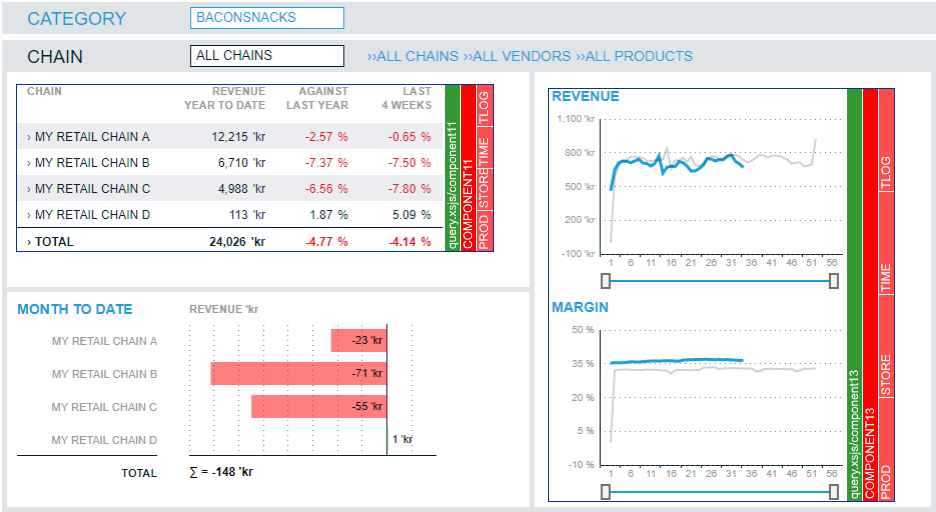
\includegraphics[width=1.00\linewidth]{pos.png}
	\caption{A section of a KPI dashboard. Directly next to UI components, elements were inserted that show which back-end functions and data sources provided the displayed data.}
	\label{fig:pos}
\end{figure}

In our prototype, mapping requests to UI components is possible because we can track from which component's ´refresh()´ method the request was sent.
As can be seen, the bar chart at the bottom left has no associated requests shown because it reuses data from the table above.
For a more generalized solution, code analysis can be used to determine to which UI components data is passed.
This will work even for scenarios where a central refresh method updates all components or where client-side post-processing of the data is performed.

Colors are used to show the involved application layers.
The green box shows the path of the request URL, the red boxes show the names of the stored procedures and database tables that where subsequently accessed.

Second, the debugger window, as shown in~\cref{fig:debugger}, shows a full overview of all interactions.
The largest part of the debugger windows is occupied by the source code.
To the right, current variable values are shown.
At the top of window, a diagram shows the entire history of all individual executions and their request/response relations.

\begin{figure}
	\centering
		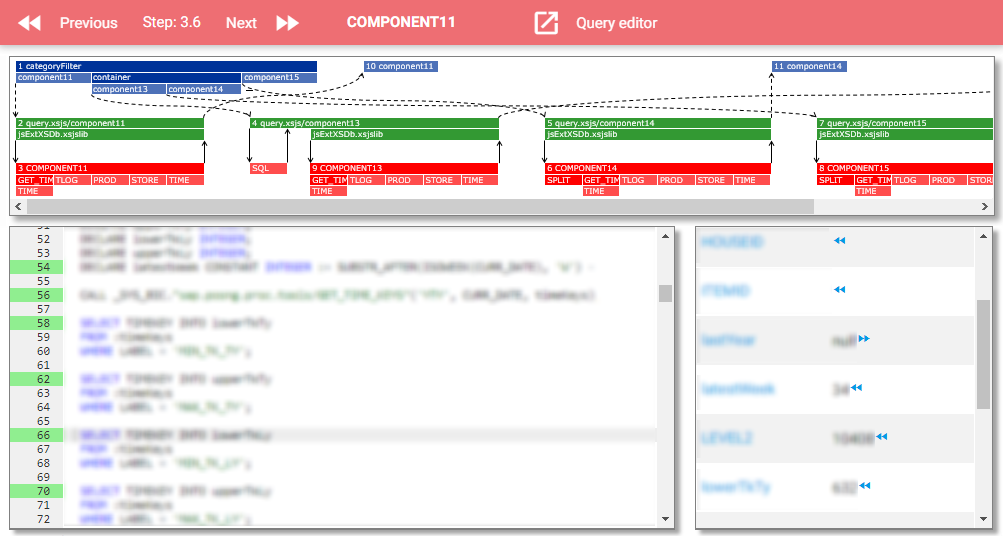
\includegraphics[width=1.00\linewidth]{debugger_full.png}
	\caption{A screenshot of our debugger prototype. On top of the code and variables view, a diagram shows the flow of requests in the application.}
	\label{fig:debugger}
\end{figure}

\begin{figure}
	\centering
		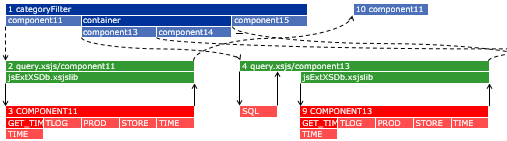
\includegraphics[width=1.00\linewidth]{executions.png}
	\caption{A part of the interaction diagram. Colors encode the application layer, dashed arrows represent asynchronous, solid arrows represent synchronous requests and responses.}
	\label{fig:executions}
\end{figure}

\Cref{fig:executions} shows a part of the interaction diagram in more detail, with anonymized names.
Each group of adjacent rectangles represents one execution trace.
The execution number and name are shown in the topmost rectangle of each group.

For the front-end, shown in blue, the blocks represent the hierarchy of UI components.
In the application layer, green blocks show the files that were executed to respond to requests and below files that submitted database queries.
Red blocks, finally, show the stored procedures that were called and, in lighter red, the tables that were accessed.
At the beginning of execution \#4 in the application layer, a plain SQL query is submitted to the database, not calling any procedures.

The length of the rectangles has no significance, in particular it does not reflect execution times.
Between the layers, asynchronous calls are shown with dashed lines, synchronous calls with solid lines.

The diagram is interactive.
For example, clicking the arrows reveals details about the requests.
For HTTP requests, the request URL and arguments and the response body are shown.
Clicking a database request opens a query window with the query string.
This allows developers to inspect the query result and to modify the query, which can help to better understand the data.
Finally, clicking a rectangle moves the debugger to the point in time where the respective code is executed.

\subsection{Debugging the Full Stack}

After developers have gained an overview over the full execution history and maybe formed first hypotheses about the bug, they want to begin debugging the code.
With the entire execution history recorded, a post-mortem debugger can replay the execution.

To identify a point in time, the debugger needs the execution number and the instruction index within the execution.
From the execution number, the debugger resolves which trace database to use.
Then, with the instruction index the current code location and program state is restored.
Stepping forwards and backwards changes the instruction index within the execution.

Typically, a back-in-time debugger allows to step forwards and backwards within a method and into and out of method calls.
When an instruction is reached that is associated with a request to another layer, 
an additional option is given to step into the execution that handles the request.
For asynchronous requests, developers can also directly jump to the execution that handles the response.
Within any request-handling execution, stepping out of the root method call moves the debug session to the instruction where the response is received.

When a higher layer sends a request down the software stack, the debugger has to decide at which point to move to the request-handling execution.
For example, developers typically don't want to debug jQuery internals or the database driver when searching a bug in the application code.
The situation becomes more complicated when the application uses a custom abstraction layer on top of the library that is used to actually send the request.
This abstraction needs to remain debuggable, because it may contain bugs, but we also want to avoid slowing down developers every time they want to follow a request.

Our debugger prototype allows developers to store a custom list of request commands, which are specified using a sub-set of XPath.
For example, a developer might specify "´//sendSQL´" to mark a method that builds and submits an SQL query string.
All method invocations that match the XPath pattern will be associated with a request, if a request was sent from within that invocation, no matter how deeply nested.
When the developer reaches such an invocation in the debugger or debugs within such an invocation, the buttons for jumping to the request and to the response handler are shown.

In our prototype, the XPath expression can contain only node names that are matched against method names, using only the child and descendants axes.
However, additional axes and predicates (e.g., to filter for methods of a certain class) could be implemented with our approach.

On top of the simplified navigation of the application stack, additional synergy effects can occur when integrating the debuggers.
Our omniscient debugger for stored procedures allows to query the database from previous points in time~\cite{treffer2017bringing}.
An extension to SQL allows developers to specify steps from the execution of the stored procedure in their queries.
We enabled the back-in-time query feature for all layers.

Developers can use hierarchical step numbers, e.g. "1.17" for the 17th step of the first execution, to select points in time in SQL queries.
A query pre-processors maps this number to a database snapshot.
If the execution number does not represent a stored procedure, the next stored procedure call is looked up by following requests from the application flow graph and the first step of that execution is used as a point-in-time.
If there is no next stored procedure call, the last step of the last previous call is used.
After that, the stored procedure steps are converted into timestamps using the mechanisms that are already in place.

Allowing to query the database from all layers has two advantages.
First, developers can look at the data while debugging the front-end.
No switching of tools is required and the database is automatically shown as it was at the respective point in time.
Second, developers can now query for changes in the data that happens across multiple executions.
For example, \cref{lst:tdiff} shows a back-in-time query that selects all products whose margin-attribute changed between the beginning of the first execution (step~1.1) and the beginning of the first response handler (step~10.1, cf.~\cref{fig:executions}).

\begin{lstlisting}[language=HanaSQL,float=t,caption={A query selecting all products whose margin was changed during the operation.},label=lst:tdiff,numbers=none]
	SELECT p.name, p.margin
	FROM Products p
  WHERE ^start!^p.margin != ^now!^p.margin
	^§AT STEP§ start=1.1, now=10.1^
\end{lstlisting}

%todo: synergy

\subsection{Developer Feedback}

We showed our debugger prototype to the developers we initially interviewed to understand the development and debugging processes in 3-tier business applications.

All developers immediately liked the idea of displaying back-end operations directly in the user interface.
Such a feature would not only be useful for debugging, but also for documentation purposes.
The developers also wished that this visualization was interactive like the interaction diagram, i.e., that clicking the boxed showed details about the requests and allowed to jump to the respective instruction in the debugger.
One developer argued that showing the back-end operations in a three dimensional stack would allow to show more details, especially in user interfaces with smaller individual components.
\Cref{fig:3d} shows a mock-up of the idea.

\begin{figure}
	\centering
		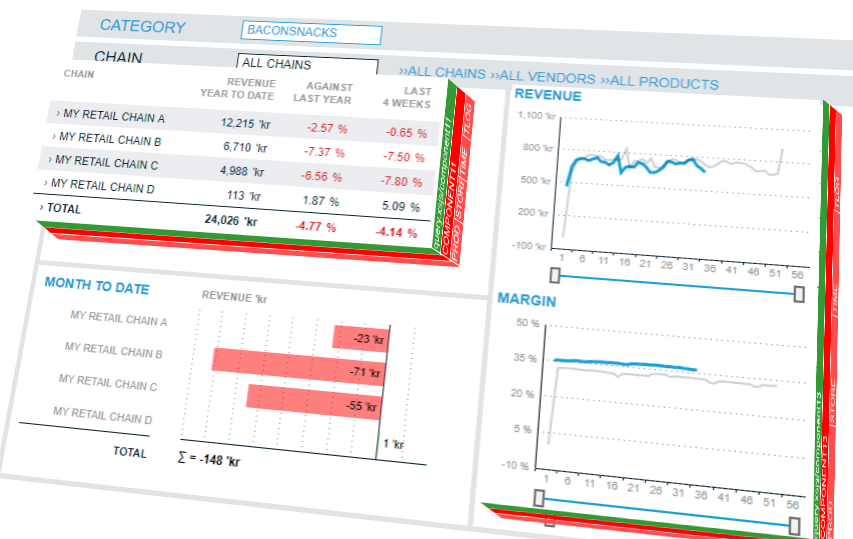
\includegraphics[width=1.00\linewidth]{pos3d.png}
	\caption{3D visualization of the software stack in the front-end. Developers can tilt the page to read debugging information on the side of the stacks.}
	\label{fig:3d}
\end{figure}

The interaction diagram was perceived as equally useful.
The developers generally liked the idea of not arranging elements based on timing related information, which allows for a clearer visualization of the logical connections between the application's sub-systems.
Compared to the network log of the browser's development tools that is typically used to get this information, this would be an improvement.
However, they also conceded that sometimes the timing of requests is important, for example when debugging performance bugs or understanding racing conditions caused by concurrent side effects.
Being able to toggle between a time-based and a logical layout would allow developers to get the best of both worlds.

Finally, all developers liked being able to go back and forth in time while following the application flow across layer boundaries.
The possibility to restart an execution without having to craft a corresponding request was already perceived as a huge improvement over existing tools.
Three developers emphasized the usefulness of being able to specify custom request methods with XPath, because they used a custom SQL query builder in their projects.

\subsection{Generalization of Our Results}

Our prototype requires that omniscient debugging is possible on each individual application layer.
However, based on the developer feedback we identified a few "low-hanging fruits" for debugging tools.
For example, developers enjoyed the visualizations of the sub-system interactions.
Collecting the necessary data for such visualizations should be easily possible with today's tools.
Many systems allow to log all requests that are sent or received and the coverage data collected by typical profiling tools is enough to restore the application flow.
Second, restarting an execution from a request can be automated.
Most requests are not large in size and can be stored for the length of a debug session, allowing developers to restart with the push of a button.
Both features combined already allow for a greatly improved debugging workflow, while no detailed tracing for back-in-time debugging is needed.
Tools like Recon or the Path Suite~\cite{lee_unified_2011, perscheid_testdriven_2013} already use automated restarting to optimize execution tracing.

We developed our debugger to work with a SAPUI5 front-end, an SAP HANA JavaScript application layer, and SAP HANA stored procedures.
To extend our prototype to support more programming languages and technologies, two problems have to be solved.
First, there must be a solution for back-in-time debugging within the respective environment, e.g., by recording detailed traces.
Second, the requests sent and received must be identifiable in such a way that they can be matched with the requests and responses collected from other layers.
Both problems are highly technology-specific. 
However, once a solution is found it can be encapsulated in a module that then extends a meta-debugger such as our prototype.

\section{Conclusion}
\label{sec:conclusion}

With the rising popularity of service-oriented architectures and micro-services in particular, the need for debugging tools that support complex heterogeneous systems is steadily increasing.
We presented a back-in-time debugger that allows the seamless debugging of a 3-tier application stack.
The feature set of our prototype was based on insights gained from interviewing developers who work on modern business applications handling large amounts of data.

Two visualizations help navigating the full execution across all layers, while individual layers can be debugged with back-in-time debugging.
We showed our prototype to developers and received promising feedback regarding the usefulness of the visualizations and their integration with a debugger.

For future work, we wish to enable code analysis across layer boundaries.
If, for example, an object in the application layer is serialized as JSON and then materialized as a JavaScript object in the front-end, an approach is needed to link the fields of both objects in a way that does not require analyzing the JSON serialization and de-serialization logic.

However, as our interviews have shown, even a basic integration of tools can already be a great improvement for developer productivity.
Modular IDEs such as Eclipse allow adding support for new programming languages and technologies via plug-ins with standardized interfaces.
Now, a similar architecture is needed for debuggers to allow not only the development, but also debugging of heterogeneous systems.


\bibliographystyle{IEEEtran}
\bibliography{references}

\end{document}
